\chapter{Utvrđivanje relativne i apsolutne lokacije u zatvorenom prostoru}
\label{chap:procjenaLokacije}

Tehnologije navigacije i pozicioniranja koje se oslanjaju na udaljene satelite (poput GPS i GNSS tehnologija) nisu pogodne za korištenje u zatvorenim prostorima iz razloga što njihove signale apsorbiraju i reflektiraju krovovi, zidovi i ostali objekti u okolini. 
Iz istih razloga određivanje lokacije preko mobilnih signala, odnosno preko radio tornjeva nije moguće. 
\\
Stoga su za utvrđivanje lokacije u zatvorenom prostoru potrebni sasvim novi i drugačiji pristupi problemu te shodno tome, sasvim nove metode određivanja lokacije. 
Zbog ogromnog porasta pristupačnosti i popularnosti pametnih telefona, posljednjih nekoliko godina sve je veća potražnja za pouzdanim rješenjem problema. 
Kako ne postoji nikakav \textit{de facto} standard, gotovo sva ponuđena rješenja su međusobno različita i koriste cijeli niz različitih tehnologija, od optičkih (npr. kamera uređaja) i radio (npr. signali obližnje bežične mreže) skroz do akustičnih (npr. akustični sljednici koji se često koriste sustavima virtualne stvarnosti) tehnologija.
\\

Vjerojatno najznačajniji uspjeh je postignut sa praćenjem signala kojega odašilje obližnja bežična Wi-fi mreža. 
Velika prednost ove metode je značajan porast bežičnih pristupnih točaka na koje se mobilni i drugi uređaji mogu spojiti. 
Da bi se ovom metodom odredila lokacija uređaja potrebno je na neki način mapirati dotičnu pristupnu točku te zatim na temelju jakosti primljenog signala utvrditi poziciju mobilnog uređaja u odnosu na nju. 
Parametri mapiranja uključuju apsolutnu poziciju, SSID\footnote{\textit{service set identification}} i MAC\footnote{\textit{media access control address}} adresu pristupne točke (tj. WLAN uređaja). 
Neke od poznatijih web aplikacija poput WeFi\footnote{\url{http://www.wefi.com/maps/}} i WiGLE\footnote{\url{https://wigle.net}} sadrže više od sto milijuna mapiranih bežičnih pristupnih točaka. 
\\

\begin{figure}
    \centering
    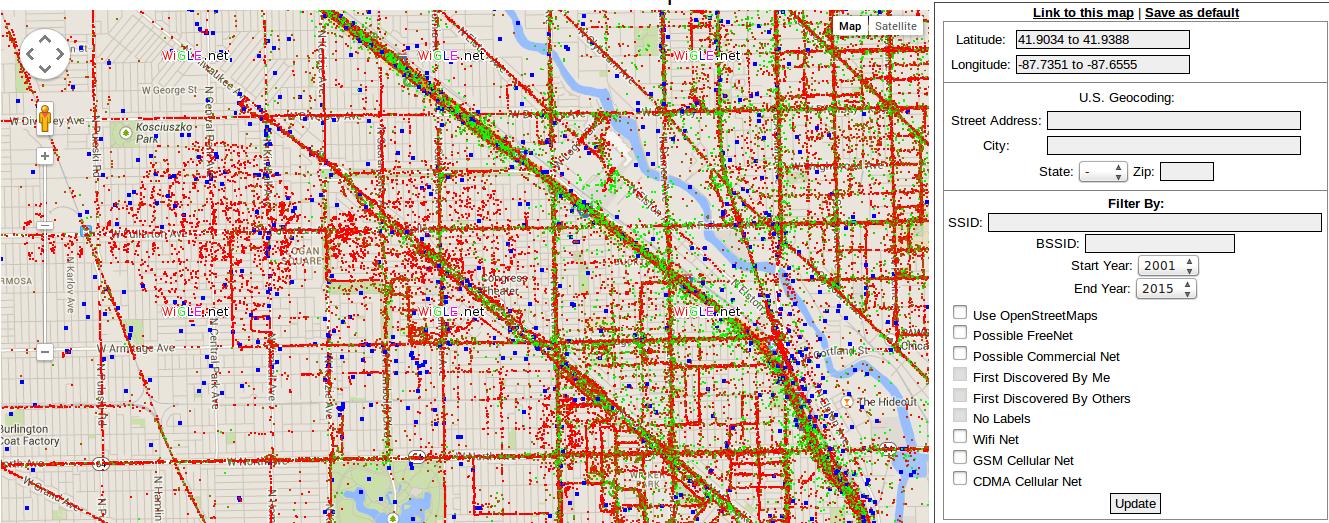
\includegraphics[scale=0.3]{pictures/WiGLE}
    \caption{Prikaz mapiranih bežičnih pristupnih točaka preko sučelja WiGLE web aplikacije}    
    %\caption{Prikaz mapiranih bežičnih pristupnih točaka kojega pruža sučelje WiGLE web aplikacije}
\end{figure}

Uz navigaciju i pozicioniranje pomoću Wi-fi mreža, dosta su popularne metode koje se služe tehnikama proširene i virtualne stvarnosti te tehnikama strojnog učenja, raspoznavanja uzoraka i računalnog vida.
\\
Jedna od popularnijih tehnika proširene \engl{augmented} i virtualne stvarnosti je korištenje posebnih oznaka (markera) kojega kamera mobilnog uređaja može prepoznati u prostoru.
\\

Iz područja strojnog učenja, raspoznavanja uzoraka i računalnog vida vjerojatno najistaknutiji i najambiciozniji projekt je projekt Tango\footnote{\url{https://www.google.com/atap/projecttango/}} kojega razvija tehnološki gigant Google. 
Cilj projekta je ponuditi rješenje koje će korištenjem kamere i ostalih senzora mobilnog uređaja nuditi pomoć pri navigaciji, pozicioniranju i prepoznavanju okoline, odnosno 3D mapiranje, u zatvorenom i otvorenom prostoru. 
Unatoč tome što je projekt još u ranoj fazi razvoja, razvojni tim je ostvario vidljiv napredak te inicijalni rezultati upućuju na preciznost od jednog centimetra. 
Uz to, prvi prototipovi mobilnih uređaja i tableta već su dostupni partnerima koji sudjeluju u razvoju i na internetu se polako objavljuju nove i zanimljive informacije o projektu. 

\begin{figure}[H]
    \centering
    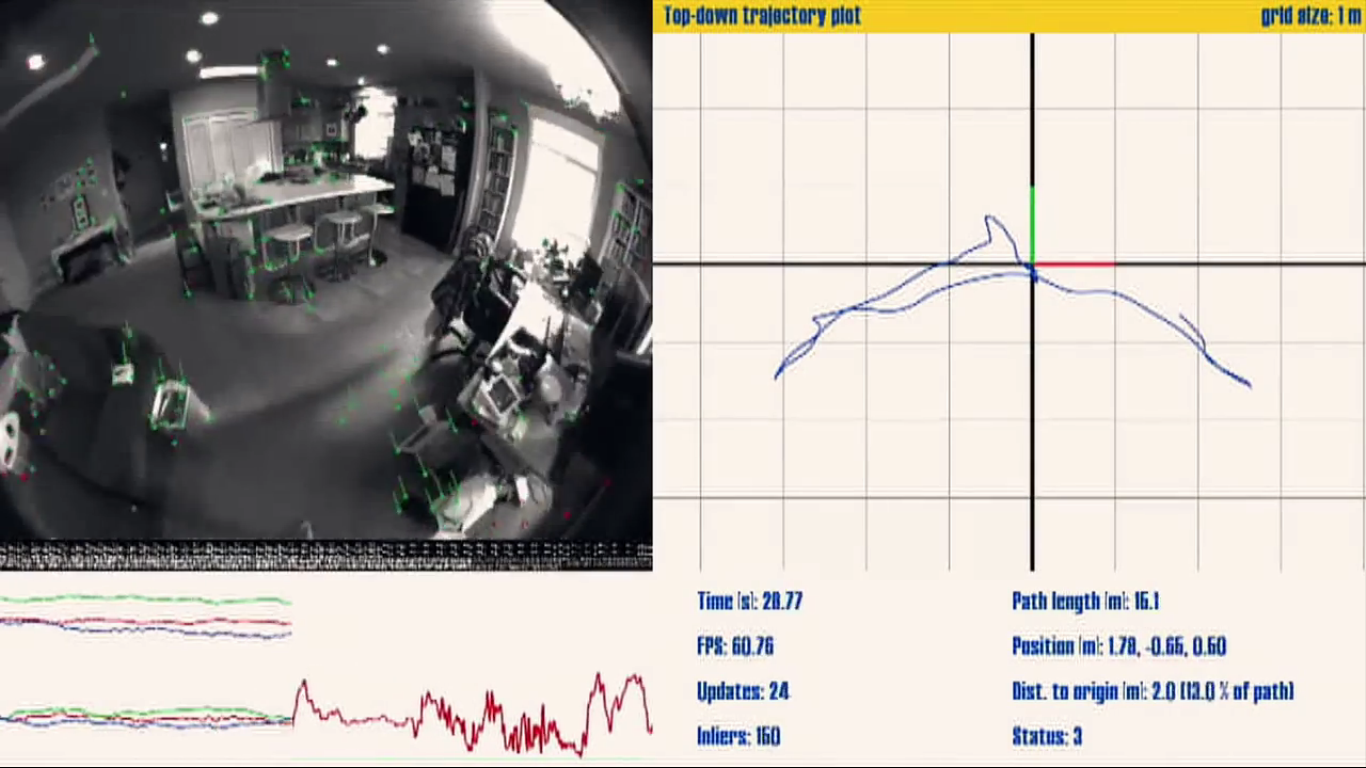
\includegraphics[scale=0.24]{pictures/tango1}
    \caption{Google Project Tango - prepoznavanje predmeta u okolini}
\end{figure}

\begin{figure}[H]
    \centering
    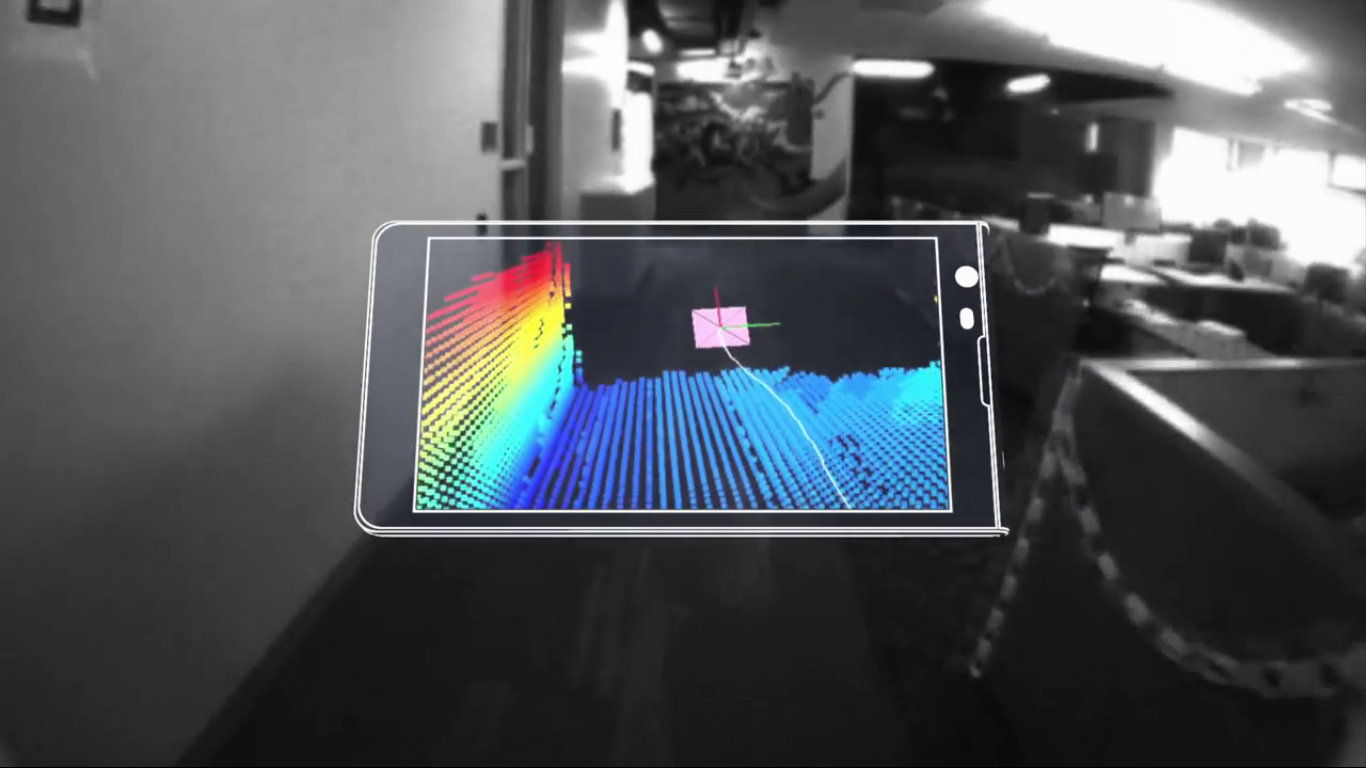
\includegraphics[scale=0.24]{pictures/tango2}
    \caption{Google Project Tango - prikaz mapirane okoline}
\end{figure}
%TODO referencirati youtube video u captionu

U nastavku su opisane relativno nove metode za određivanje lokacije u zatvorenom prostoru koje se temelje na BLE tehnologiji i iBeacon odašiljačima.
Za rješavanje problema prvo je potrebno sa što većom preciznošću odrediti relativnu poziciju uređaja u odnosu na odašiljač/odašiljače stoga je glavni fokus istraživanja usmjeren baš na taj dio. 
Nakon toga uz poznavanje relativne pozicije uređaja i apsolutne pozicije odašiljača možemo odrediti apsolutni položaj uređaja.

\section*{Utvrđivanje relativne udaljenosti od odašiljača}

Funkcija pomoću koje se može odrediti jakost primljenog signala navedena je u \eqref{eq:procjenaSignala}.

\begin{equation}
	\label{eq:procjenaSignala}
	P_r = P_t + 20\log{\frac{\lambda}{4\pi}} + 10n\log{\frac{1}{d}}
\end{equation}

$P_t$ predstavlja jakost odašiljanja signala, $P_r$ jakost primljenog signala, $d$ udaljenost između prijamnika i odašiljača, $\lambda$ je valna duljina elektromagnetskog vala, a $n$ indeks refrakcije (u slobodnom prostoru iznosi 2).
\\

Ukoliko se ista jednadžba zapiše po varijabli $d$ dobiva se formula koja je prikazana u \eqref{eq:procjenaUdaljenosti}. 
Uz poznate vrijednosti svih ostalih parametara ta formula se može iskoristiti za procjenu udaljenosti između prijamnika i odašiljača.
Uz to, zbog relativno niske složenosti dotična formula je idealan kandidat za ugradnju u mobilnu aplikaciju.

\begin{equation}
	\label{eq:procjenaUdaljenosti}
	d = 10^{-\frac{P_r - P_t - 20\log{\frac{\lambda}{4\pi}}}{10n}}
\end{equation}

Problem formule \eqref{eq:procjenaUdaljenosti} je što ona zanemaruje bilo kakva ometanja signala, odnosno ona je ona primjenjiva samo u idealnim uvjetima, a kao što je prethodno već rečeno, na signal u zatvorenom prostoru utječe (tj. ometa ga) velik broj parametara. 
Na stabilnost signala koji putuje zatvorenim prostorom najvećim dijelom djeluju apsorpcija i refleksija signala, dok razašiljanje i difrakcija djeluju manjom mjerom.
\\
Zbog refleksije signala dio elektromagnetskog vala se odbija (reflektira) od površinu s kojom se sudario, a zbog apsorpcije signala dio elektromagnetskog vala se apsorbira te se val nastavlja gibati sa prigušenjem. 
%Ukupni gubitak jednak je zbroju pojedinih gubitaka. 
Smetnje uzrokovane refleksijom mogu se smanjiti povećanjem frekvencije, dok apsorpcija ovisi o dubini prodiranja i udaljenosti granice između dva sredstva. 
\\

U zatvorenom prostoru smetnje koje uzrokuju prethodno opisani faktori su često prevelike i u velikoj većini slučajeva na to se ne može utjecati. 
Zaključak je da procjena udaljenosti temeljena na \eqref{eq:procjenaUdaljenosti} nije precizna na tako nestabilnom signalu stoga je za rješavanje problema potreban drugačiji pristup.
\\

Sustav za procjenu udaljenosti od iBeacon odašiljača može se opisati kao što je prikazano na slici\ref{fig:sustavZaProcjenuUdaljenosti}.

\begin{figure}[H]
    \centering
    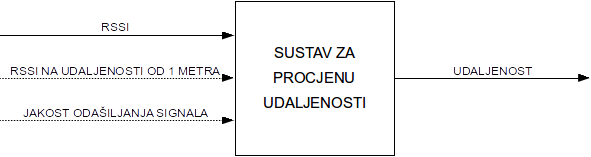
\includegraphics[scale=0.68]{pictures/sustav-za-procjenu-udaljenosti}
    \caption{Sustav za procjenu udaljenosti}
    \label{fig:sustavZaProcjenuUdaljenosti}
\end{figure}

Ulaz u sustav procjene udaljenosti je RSSI, odnosno jakost primljenog signala, opcionalni ulazni parametri su jakost odašiljanja signala te RSSI izmjeren na udaljenosti od jednog metra od odašiljača, a izlaz sustava je procjena udaljenosti izražena u metrima.
\\
Sustav procjene udaljenosti može biti funkcija \eqref{eq:procjenaUdaljenosti} ili bilo koja druga funkcija.
\\
Kako na signal djeluje velik broj vanjskih smetnji, predloženi sustav će morati biti otporan na šum u podacima, a također će morati biti i relativno brz te imati nisku složenost zbog toga što mu je primarna namjena korištenje u mobilnim uređajima i tabletima ograničene procesorske snage. 
\\

Kao što je navedeno u iBeacon poglavlju, Apple je za procjenu udaljenosti od odašiljača namijenio tri izraza: neposredna blizina (\textit{immediate}), mala (\textit{near}) i velika \textit{far} udaljenost.
Zajedno s tim u radno okruženje Apple Core Location dodana je funkcija koja na temelju jakosti primljenog signala (RSSI) i jakosti signala na udaljenosti jednog metra od odašiljača (trideseti bajt \textit{advertising} paketa iBeacon odašiljača) određuje relativnu udaljenost od odašiljača. 
Sam kôd funkcije nije javno dostupan i nije poznata metoda koju su Appleovi inženjeri upotrijebili, no \textbf{ne preporučuju} da se ona koristi u situacijama gdje je potreban precizan rezultat, odnosno precizna procjena udaljenosti. 
Stoga se nameće zaključak kako ni Appleovi inženjeri nisu uspjeli zaobići prethodno spomenute smetnje koje djeluju na signal.
\\

Inženjeri američke kompanije Radius Networks su za vrijeme izrade svoje neslužbene slobodno dostupne Android iBeacon biblioteke\footnote{\url{https://github.com/RadiusNetworks/android-ibeacon-service}} pristupili problemu procjene udaljenosti tako da su napravili veliki broj RSSI mjerenja na poznatim udaljenostima i rezultate opisali funkcijom najbolje sličnosti \citep{stackoverflowRadiusDistancing}. 
Dotična funkcija navedena je u \eqref{eq:rnFunkcija}.

\begin{equation}
	\label{eq:rnFunkcija}
	f(x,y) = 
	\begin{cases}	
	0.89976 {\dfrac{x}{y}}^{7.7095} + 0.111 & \text{ako } \dfrac{x}{y} \geq 1 \\
	{\dfrac{x}{y}}^{10} & \text{ako } 0 < \dfrac{x}{y} < 1 \\
	-1 & \text{ako } x = 0 	
	\end{cases}
\end{equation}
\\

Parametar $x$ je RSSI primljenog signala, dok $y$ predstavlja RSSI na udaljenosti od jednog metra od odašiljača. 
\\

Njihovo rješenje može se isprobati tako da se funkciju \eqref{eq:rnFunkcija} ugradi u vlastitu aplikaciju, a može se iskoristiti i njihova besplatna Android aplikacija koja je dostupna na Google Play Storeu\footnote{\url{https://play.google.com/store/apps/details?id=com.radiusnetworks.ibeaconlocate}}.
\\
Empirijskim testiranjem aplikacije primjetio sam kako i za male pomake u iznosu od nekoliko desetaka centimetara detektirani pomak aplikacije nerijetko bio u iznosu većem od deset metara. 
Stoga se može zaključiti kako ni rješenje koje su ponudili inženjeri Radius Networksa nije pouzdano, a ni primjenjivo na stvarnim problemima. 
Bez obzira na to, njihova Android iBeacon biblioteka, objašnjenja na službenim stranicama te rasprave njihovog inženjera David Younga na stranicama Stackoverflowa su izuzetno pomogle oko shvaćanja cjelokupne problematike određivanja lokacije korištenjem iBeacon odašiljača.
\\

Kao model sustava možemo iskoristiti umjetnu neuronsku mrežu \engl{artificial neural network}.  
Smatram da su neuronske mreže dobar model za rješavanje problema iz razloga što one mogu uspješno rješavati zahtjevne probleme gdje je tražena funkcija nepoznata, a uz to otporne su otporne na šum u podacima. 
Daljnji rad će se zasnivati na korištenju unaprijedne neuronske mreže, iako bi se za rješavanje problema mogla koristiti i neizrazita neuronska mreža.
\\

Neuronska mreža će se trenirati na prethodno prikupljenim podacima. 
Prve tri skupine podataka uzorokovane su na na udaljenostima od \SI{50}{cm} do \SI{8}{m} s korakom od \SI{50}{cm}, po dvije stotine uzoraka za svaku udaljenosti. 
Ukupno prve tri skupine sastoje se od $brojSkupina \cdot brojUdaljenosti \cdot brojUzoraka = 3 \cdot 16 \cdot 200 = 9600$ nezavisnih uzoraka. 
Važnija svojstva sve tri skupine uzoraka prikazane su u tablicama \ref{tbl:indoorKontaktDefaultTx}, \ref{tbl:indoorKontaktMaxTx} i \ref{tbl:blucatsDefault}.

\begin{table}[H]
	\centering
	\caption{Uzorci koje je KontaktIO iBeacon saTODO}
	\label{tbl:indoorKontaktDefaultTx}
	\begin{tabular}{ccccc}
	\hline
	Udaljenost & $\mu_{RSSI}$ & $\sigma_{RSSI}$ & $min_{RSSI}$ & $max_{RSSI}$ \\
	\hline
	0.5 & -81.075 & 2.426 & -88 & -74 \\
	1.0 & -80.320 & 2.799 & -86 & -76 \\
	1.5 & -75.575 & 3.298 & -80 & -70 \\
	2.0 & -73.990 & 2.558 & -79 & -68 \\
	2.5 & -78.725 & 0.907 & -81 & -74 \\
	3.0 & -82.470 & 4.053 & -91 & -74 \\
	3.5 & -81.685 & 2.892 & -87 & -77 \\
	4.0 & -83.115 & 1.903 & -88 & -77 \\
	4.5 & -91.125 & 3.057 & -98 & -85 \\
	5.0 & -88.705 & 2.198 & -93 & -83 \\
	5.5 & -88.935 & 3.487 & -97 & -83 \\
	6.0 & -92.450 & 2.399 & -99 & -87 \\
	6.5 & -93-610 & 1.691 & -99 & -90 \\
	7.0 & - & - & - & - \\
	7.5 & - & - & - & - \\
	8.0 & - & - & - & - \\
	\hline
	\end{tabular}
\end{table}

%TODO opisati rezultat tablice, priložiti pripadni graf, obrazložiti graf

\begin{table}
	\centering
	\caption{TODO}
	\label{tbl:indoorKontaktMaxTx}
	\begin{tabular}{ccccc}
	\hline 
	Udaljenost & $\mu_{RSSI}$ & $\sigma_{RSSI}$ & $min_{RSSI}$ & $max_{RSSI}$ \\ 
	\hline 
	0.5 & -65.165 & 2.546 & -76 & -56 \\
	1.0 & -66.250 & 2.316 & -73 & -59 \\
	1.5 & -62.695 & 4.3238 & -69 & -57 \\
	2.0 & -58.750 & 1.982 & -62 & -53 \\
	2.5 & -63.595 & 0.875 & -66 & -59 \\
	3.0 & -67.810 & 2.619 & -73 & -62 \\
	3.5 & -71.620 & 3.537 & -80 & -65 \\
	4.0 & -68.72 & 2.000 & -73 & -65 \\
	4.5 & -74.975 & 3.065 & -81 & -68 \\
	5.0 & -72.445 & 3.485 & -78 & -65 \\
	5.5 & -79.920 & 6.883 & -93 & -68 \\
	6.0 & -82.175 & 5.896 & -98 & -71 \\
	6.5 & -74.085 & 2.977 & -80 & -68 \\
	7.0 & -71.700 & 2.858 & -77 & -65 \\
	7.5 & -76.065 & 2.241 & -80 & -71 \\
	8.0 & -78.295 & 4.926 & -91 & -71 \\
	\hline
	\end{tabular}
\end{table}

%TODO opisati rezultat tablice, priložiti pripadni graf, obrazložiti graf

\begin{table}
	\centering
	\caption{TODO}
	\label{tbl:blucatsDefault}
	\begin{tabular}{ccccc}
	\hline
	Udaljenost & $\mu_{RSSI}$ & $\sigma_{RSSI}$ & $min_{RSSI}$ & $max_{RSSI}$ \\
	\hline
	0.5 & -89.550 & 3.526 & -98 & -83 \\
	1.0 & -90.895 & 2.101 & -96 & -86 \\
	1.5 & -91.350 & 3.162 & -101 & -86 \\
	2.0 & -91.695 & 2.134 & -99 & -86 \\
	2.5 & -89.630 & 1.583 & -99 & -86 \\
	3.0 & -93.385 & 2.156 & -100 & -88 \\
	3.5 & - & - & - & - \\
	4.0 & - & - & - & - \\
	4.5 & - & - & - & - \\
	5.0 & - & - & - & - \\
	5.5 & - & - & - & - \\
	6.0 & - & - & - & - \\
	6.5 & - & - & - & - \\
	7.0 & - & - & - & - \\
	7.5 & - & - & - & - \\
	8.0 & - & - & - & - \\
	\hline
	\end{tabular}
\end{table}

%TODO opisati rezultat tablice, priložiti pripadni graf, obrazložiti graf


%TODO mjerenja na većoj udaljenosti - tablica + graf

\begin{table}
    \centering
    \caption{TODO}
    \label{tbl:velikaUdaljenost}
    \begin{tabular}{ccccc}
    \hline 
    Udaljenost & $\mu_{RSSI}$ & $\sigma_{RSSI}$ & $min_{RSSI}$ & $max_{RSSI}$ \\ 
    \hline 
    2 & -63.720 & 1.371 & -66 & -59 \\ 
    4 & -72.755 & 4.294 & -80 & -67 \\ 
    6 & -74.450 & 6.894 & -89 & -65 \\ 
    8 & -77.300 & 2.112 & -83 & -71 \\ 
    10 & -83.905 & 4.691 & -92 & -77 \\ 
    12 & -84.265 & 3.489 & -95 & -77 \\ 
    14 & -85.580 & 2.430 & -90 & -81 \\ 
    16 & -90.560 & 2.846 & -97 & -85 \\ 
    18 & -92.555 & 1.787 & -98 & -88 \\ 
    20 & -87.395 & 3.157 & -93 & -83 \\ 
    22 & -92.375 & 2.7988 & -99 & -86 \\ 
    24 & -91.53 & 1.407 & -95 & -88 \\ 
    \hline 
    \end{tabular} 
\end{table}


%TODO postupci: matematički, best fit curve, neuronska mreža i poteškoće, spomeniti genetsko programiranje
%TODO zaključak



\section*{Utvrđivanje apsolutne lokacije}
%TODO općenito o utvrđivanju apsolutne lokacije

\subsection*{Triangulacija}

Postupak triangulacije
%TODO objasniti postupak triangulacije
%TODO matematički postupak kod triangulacije
%TODO iBeacon i triangulacija

\subsection*{Trilateracija}
%TODO objasniti postupak trilateracije
%TODO matematički postupak trilateracije
%TODO iBeacon i trilateracija